\documentclass[tikz,border=10pt]{standalone}
\usetikzlibrary{angles,quotes,calc}
\begin{document}
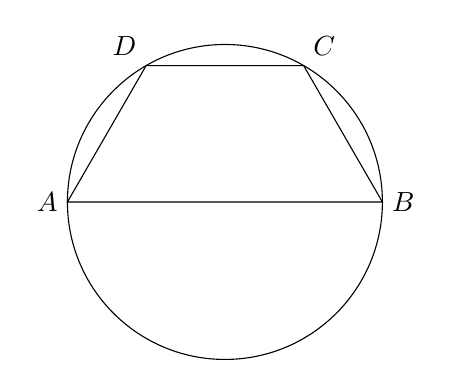
\begin{tikzpicture}    
% 定义参数    
\def\R{2} % 圆半径    
\def\angleC{60} % 点C的角度，可调节    
\def\angleD{120} % 点D的角度，可调节
    % 绘制圆    
\draw (0,0) circle (\R);
    % 定义坐标点    
\coordinate (O) at (0,0);    
\coordinate (A) at (-\R,0);    
\coordinate (B) at (\R,0);    
\coordinate (C) at (\angleC:\R);    
\coordinate (D) at (\angleD:\R);    
\coordinate (E) at ($(A)!(C)!(B)$); % E点为C在AB上的投影
    % 绘制梯形边    
\draw (A) -- (B) -- (C) -- (D) -- cycle;


    % 标注点标签    
\node[left] at (A) {$A$};    
\node[right] at (B) {$B$};    
\node[above right] at (C) {$C$};    
\node[above left] at (D) {$D$}; 
\end{tikzpicture}
\end{document}